\chapter{Ablation Study}
\label{chap:ablation}
\chaptermark{Ablation Study}

This chapter examines how much of the reference model's input context and
feed-forward capacity can be removed while retaining detection performance.
We vary window length and feed-forward width without changing the
encoder--decoder structure of TranAD+. The study separates reductions in
learned parameter storage from reductions in arithmetic work, then relates
both to the recorded detection metrics.

The results do not follow a universal compression--accuracy curve.
The joint reduction is favorable on \ac{OPS-SAT} and \ac{SMAP}, whereas
\ac{MSL} combines stable \ac{POT} performance with substantial variability
in the original Best F1 search. These differences are examined within each
dataset before drawing conclusions across datasets.

\section{Experimental design}
\label{sec:ablation-design}
The study uses the complete two-pass TranAD+ implementation described in
Section~\ref{sec:background-tranadplus-training} and the reference
code~\cite{TranADPlusReferenceCode}. The changed quantities
are window length \(w\) and effective feed-forward width
\(d_{\mathrm{ff}}\). All other model dimensions remain fixed within a
dataset. In particular, reducing \(w\) does not remove input features or
change the number of encoder and decoder stacks.

Table~\ref{tab:ablation-design} lists the effective integer grids. Each
of the \num{30} settings per dataset is trained with seeds
\num{2026}, \num{2027} and \num{2028}, giving \num{270} runs in total.
All runs use \num{50} epochs and one layer per Transformer stack.
The grids are expressed in actual dimensions, since rounding fractional
settings can otherwise obscure which models are being compared.

\begin{table}[htbp]
  \centering
  \small
  \setlength{\tabcolsep}{5pt}
  \begin{tabular}{@{}lrlrrrr@{}}
    \toprule
    Dataset & \(F\) & Window grid & FF grid & \(B\) & \(\eta\) & \(q\) \\
    \midrule
    \acs{OPS-SAT} & \num{1} & \(3,4,5,6,8,10\) & \(2,3,4,6,8\) & \num{256} & \num{0.001} & \num{0.01} \\
    \acs{SMAP} & \num{25} & \(3,4,5,6,8,10\) & \(13,25,32,38,50\) & \num{1024} & \num{0.001} & \num{0.07} \\
    \acs{MSL} & \num{55} & \(13,25,32,38,44,50\) & \(28,55,69,83,110\) & \num{128} & \num{0.0001} & \num{0.01} \\
    \bottomrule
  \end{tabular}
  \caption{Hyperparameter-ablation design. Here \(F\) is the feature count,
  \(B\) the training batch size, \(\eta\) the initial learning rate and
  \(q\) the supplied \acs{POT} risk parameter. Each grid cell contains
  \num{3} trained seeds. Padding and scaling are enabled; batches are
  ordered and no downsampling is applied.}
  \label{tab:ablation-design}
\end{table}
% Sources: data/chapter5/runs.csv and evidence.json; all270 original reports
% verified by scripts/prepare_chapter5.py. This is the hyperparameter grid,
% not the later four-setting architectural grid in Table3.3.

The first campaign supplied \num{16} cells per dataset, and the second
added \num{14} disjoint cells to complete the grid. The model source hash
is identical throughout. The recorded evaluation or runner revisions,
however, differ between campaigns; matching model hashes alone do not
establish numerical identity of the entire pipeline. We verified the
reported metric definitions, effective settings and stored scalar results.
The principal endpoint comparisons below all belong to the first campaign,
so their contrasts do not depend on crossing those revisions. The full
combined grid provides a broader descriptive overview.
% Sources: results/analysis_v10_v12/provenance.json; original integrated
% reports' source fields. Endpoint source campaign is asserted as v10.

The primary detection result is BF200, using the original
\num{200}-threshold search with point adjustment. \ac{POT} supplies a
complementary threshold procedure. Both methods retain their own
F1-selected alpha and threshold. Precision, recall and AUC-PA are evaluated
at those same selections, rather than optimized independently.
AUC-PA retains the binary-after-adjustment definition of
Equation~\eqref{eq:datasets-binary-auc}. The training and test protocols
remain those of Chapter~\ref{chap:datasets}.

\section{Reference settings and comparisons}
\label{sec:ablation-controls}
For each dataset, the reference uses the largest window and feed-forward
width in Table~\ref{tab:ablation-design}. Its coordinates are
\((\num{10},\num{8})\) for \ac{OPS-SAT},
\((\num{10},\num{50})\) for \ac{SMAP}, and
\((\num{50},\num{110})\) for \ac{MSL}.
These are study controls, not the configurations selected for agreement
with the paper in Chapter~\ref{chap:replication}.

We examine four corners of each grid: the reference; the smallest window
at reference width; the smallest width at reference window; and the joint
minimum. These cases are defined by geometry, not by selecting the largest
test F1. Table~\ref{tab:ablation-endpoints} reports every case using the
mean and sample standard deviation across the three seeds. The full
BF200 grid and its variability are shown in
Figure~\ref{fig:ablation-grid}.

\begin{table}[htbp]
  \centering
  \small
  \setlength{\tabcolsep}{7pt}
  % Generated by scripts/prepare_chapter5.py from data/chapter5/runs.csv.
\begin{tabular}{@{}llrrrr@{}}
\toprule
Dataset & Reduction & \(w\) & \(d_{\mathrm{ff}}\) & BF200 F1 & \acs{POT} F1 \\
\midrule
\acs{OPS-SAT} & Reference & \num{10} & \num{8} & \(\num{88.34}\pm\num{0.58}\) & \(\num{65.74}\pm\num{3.01}\) \\
\acs{OPS-SAT} & Window only & \num{3} & \num{8} & \(\num{84.59}\pm\num{6.61}\) & \(\num{72.31}\pm\num{22.51}\) \\
\acs{OPS-SAT} & FF only & \num{10} & \num{2} & \(\num{84.05}\pm\num{7.46}\) & \(\num{56.54}\pm\num{8.31}\) \\
\acs{OPS-SAT} & Joint & \num{3} & \num{2} & \(\num{91.28}\pm\num{0.18}\) & \(\num{88.49}\pm\num{0.85}\) \\
\addlinespace
\acs{SMAP} & Reference & \num{10} & \num{50} & \(\num{82.90}\pm\num{1.06}\) & \(\num{81.38}\pm\num{0.98}\) \\
\acs{SMAP} & Window only & \num{3} & \num{50} & \(\num{85.26}\pm\num{0.63}\) & \(\num{84.53}\pm\num{0.09}\) \\
\acs{SMAP} & FF only & \num{10} & \num{13} & \(\num{83.88}\pm\num{1.03}\) & \(\num{81.92}\pm\num{0.22}\) \\
\acs{SMAP} & Joint & \num{3} & \num{13} & \(\num{85.76}\pm\num{0.15}\) & \(\num{84.55}\pm\num{0.09}\) \\
\addlinespace
\acs{MSL} & Reference & \num{50} & \num{110} & \(\num{51.26}\pm\num{17.61}\) & \(\num{85.69}\pm\num{0.22}\) \\
\acs{MSL} & Window only & \num{13} & \num{110} & \(\num{73.71}\pm\num{3.41}\) & \(\num{85.56}\pm\num{0.65}\) \\
\acs{MSL} & FF only & \num{50} & \num{28} & \(\num{47.62}\pm\num{21.56}\) & \(\num{85.61}\pm\num{0.58}\) \\
\acs{MSL} & Joint & \num{13} & \num{28} & \(\num{72.26}\pm\num{16.53}\) & \(\num{85.71}\pm\num{0.78}\) \\
\bottomrule
\end{tabular}

  \caption{Detection at the four grid corners. F1 is reported as
  mean \(\pm\) sample standard deviation, in percent, across \num{3} seeds.
  All entries use point adjustment and all endpoint runs belong to the
  first campaign. These are fixed-setting summaries, not best-seed values.}
  \label{tab:ablation-endpoints}
\end{table}

Two controls qualify the interpretation. First, thresholds and alpha are
reselected for each trained model according to the reference protocol.
The comparison therefore measures the response of the complete detection
pipeline, rather than the effect of changing a representation under one
frozen decision rule.

Second, the nominal optimization fragments, validation fragments and test
fragments are fixed for \ac{OPS-SAT}, and each fragment supplies the same
number of reconstruction targets at every window length. For
\ac{SMAP} and \ac{MSL}, the physical tracks are fixed, but the native
padding convention changes the number of duplicated targets with \(w\),
as specified in Equation~\eqref{eq:datasets-native-window-count}.
It can also change the number of minibatches per epoch. Consequently,
fixed epoch count does not imply exactly equal optimization-step counts,
and the native window sweep is not exclusively a change in physical
history length. These effects are retained as part of the reference
protocol.

\begin{figure}[htbp]
  \centering
  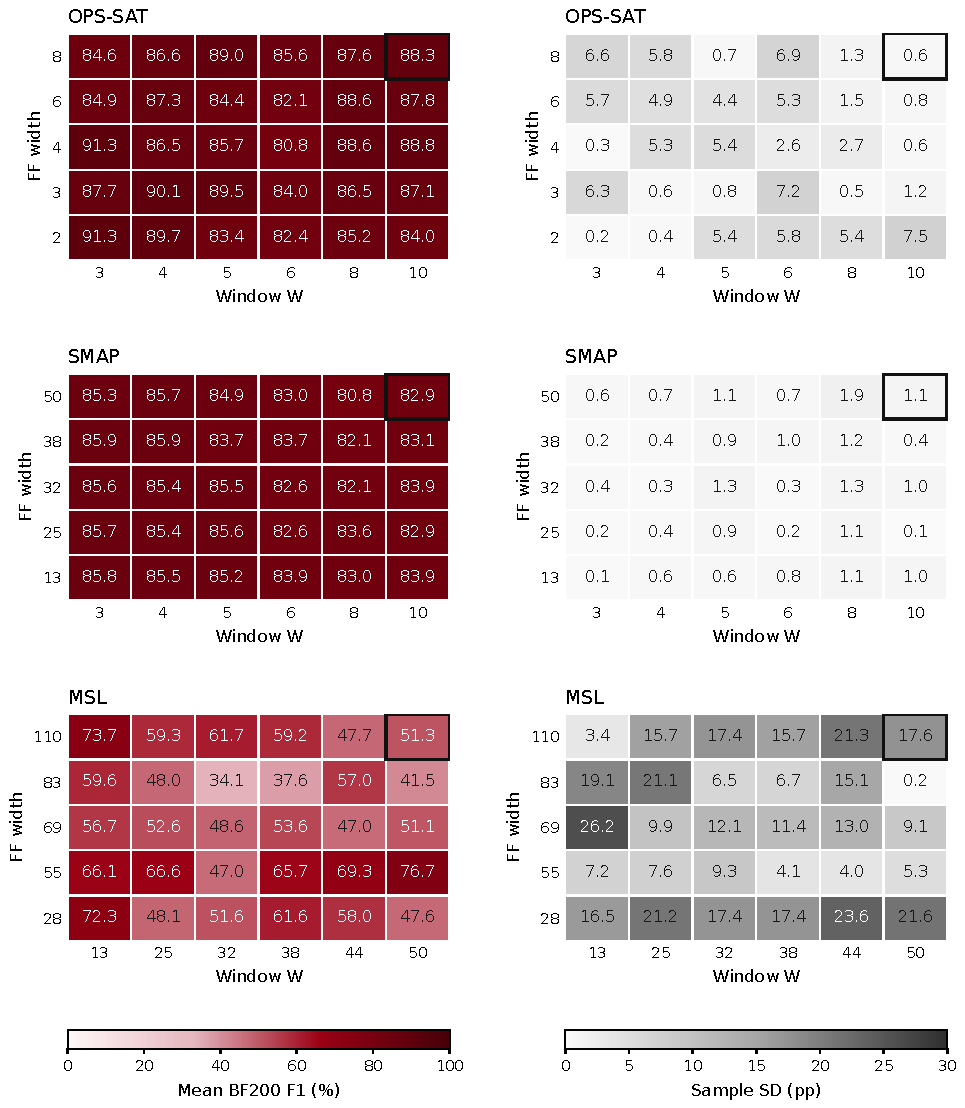
\includegraphics[width=\linewidth]{chapter5/grid_bf200.pdf}
  \caption{BF200 F1 over the complete window/width grid. Left panels show
  three-seed means in percent; right panels show sample standard deviations
  in percentage points at the same coordinates. Outlined cells are the
  largest-window, largest-width reference settings. Mean and variability
  scales are shared across datasets within their respective columns.
  The overview contains both recorded campaigns; the endpoint comparisons
  in Table~\ref{tab:ablation-endpoints} use the first campaign only.}
  \label{fig:ablation-grid}
\end{figure}
% Generated by scripts/plot_chapter5.py from verified data/chapter5/runs.csv.
% Left mean/right SD explicitly display uncertainty for each grid cell.

\section{Window-size reduction}
\label{sec:ablation-window}
The left column of Figure~\ref{fig:ablation-slices} varies the window while
holding feed-forward width at its largest value. This comparison shows
that shorter windows can be useful, but their effect depends on the
dataset and on threshold selection.

For \ac{OPS-SAT}, shortening the window from \num{10} to \num{3} at
width \num{8} lowers mean BF200 F1 from
\(\num{88.34}\pm\num{0.58}\) to
\(\num{84.59}\pm\num{6.61}\) percent. Mean \ac{POT} F1 increases
from \(\num{65.74}\pm\num{3.01}\) to
\(\num{72.31}\pm\num{22.51}\) percent, with a much wider seed spread.
The intermediate windows also depart from a monotonic trend. Window
reduction alone therefore does not establish a stable improvement on this
reference application.

For \ac{SMAP}, the same window change at width \num{50} raises mean
BF200 F1 from \SI{82.90}{\percent} to \SI{85.26}{\percent} and mean
\ac{POT} F1 from \SI{81.38}{\percent} to \SI{84.53}{\percent}.
The endpoint improvement is positive for each matched seed under both
methods. This is stronger evidence for a useful shorter-window setting,
although it is still conditional on the fixed dataset and evaluation
protocol.

For \ac{MSL}, shortening \num{50} samples to \num{13} at width
\num{110} raises mean BF200 F1 from \SI{51.26}{\percent} to
\SI{73.71}{\percent}. In contrast, \ac{POT} remains close to
\SI{85.6}{\percent} at both endpoints. The large BF200 change is not
mirrored by the alternative threshold method, so it should not be
interpreted as a threshold-independent improvement in detection.

A shorter window is not necessarily an information disadvantage for this
reconstruction task. The current sample remains in the encoder input and
the decoder query, as described in
Section~\ref{sec:background-tranadplus-training}. Reducing past context
therefore preserves direct access to the reconstruction target. It may
reduce interference from earlier conditions, while also reducing attention
work. This is a plausible computational explanation; the observed F1
values do not identify a physical correlation time in the telemetry.

\begin{figure}[htbp]
  \centering
  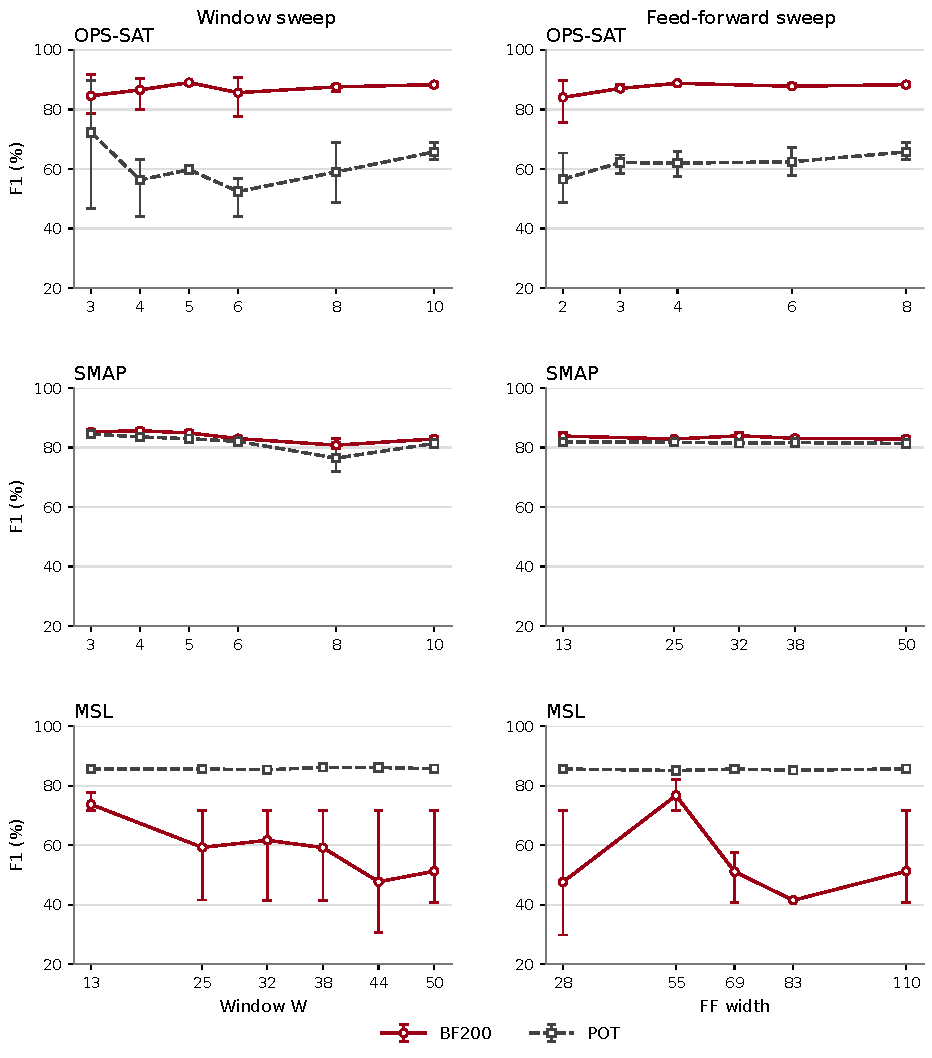
\includegraphics[width=\linewidth]{chapter5/slices_bf200_pot.pdf}
  \caption{Single-factor sweeps with point adjustment. Left: window length
  varies at the largest feed-forward width; right: feed-forward width
  varies at the largest window. The fixed widths are \num{8}, \num{50}
  and \num{110}, and the fixed windows are \num{10}, \num{10} and
  \num{50}, respectively, for \acs{OPS-SAT}, \acs{SMAP} and \acs{MSL}.
  Points are three-seed means; bars span the observed minimum and maximum.
  Lines connect sampled settings as visual guides. Both recorded campaigns
  contribute intermediate settings.}
  \label{fig:ablation-slices}
\end{figure}

\section{Feed-forward reduction}
\label{sec:ablation-feedforward}
The right column of Figure~\ref{fig:ablation-slices} holds the largest
window fixed and reduces the feed-forward width. Unlike window length,
this intervention directly reduces the number of learned weights.
The embedding width and attention-head count remain fixed, so it does
not shrink every part of the model.

For \ac{OPS-SAT}, reducing width from \num{8} to \num{2} at window
\num{10} lowers mean BF200 F1 from \SI{88.34}{\percent} to
\SI{84.05}{\percent}. Mean \ac{POT} F1 falls from
\SI{65.74}{\percent} to \SI{56.54}{\percent}.
The seed variability also increases. At this window length, the smallest
feed-forward map therefore has a measurable detection cost in the
recorded summaries.

For \ac{SMAP}, width \num{13} at window \num{10} gives BF200
\(\num{83.88}\pm\num{1.03}\) percent and \ac{POT}
\(\num{81.92}\pm\num{0.22}\) percent, compared with
\(\num{82.90}\pm\num{1.06}\) and
\(\num{81.38}\pm\num{0.98}\) percent at width \num{50}.
These changes are smaller than those produced by the window endpoints.
The sweep supports a substantial width reduction without a systematic
loss in these metrics.

For \ac{MSL}, \ac{POT} again stays near \SI{85.6}{\percent} as the
width changes. BF200 is much less stable: the largest and smallest widths
give \(\num{51.26}\pm\num{17.61}\) and
\(\num{47.62}\pm\num{21.56}\) percent. The intermediate width
\num{55} also behaves differently from neighboring widths in
Figure~\ref{fig:ablation-slices}. These observations do not support a
smooth monotonic relation between width and detection performance.

Reducing capacity can affect nominal and anomalous reconstruction errors
in different ways. A smaller reconstruction map can constrain which
patterns are reproduced, rather than merely increasing every error by
the same amount. As discussed in
Section~\ref{sec:background-reconstruction}, good reconstruction and good
anomaly separation are different objectives. The present comparisons
are consistent with that distinction, but do not by themselves demonstrate
that a wider model overfits.

\section{Joint reduction and interaction}
\label{sec:ablation-joint}
The joint endpoints reveal behavior that the isolated sweeps do not
predict. On \ac{OPS-SAT}, the smallest window and width together give
BF200 \(\num{91.28}\pm\num{0.18}\) percent and \ac{POT}
\(\num{88.49}\pm\num{0.85}\) percent. Both exceed the reference
means, although reducing either coordinate alone does not improve both
methods. The joint-minus-reference F1 differences are positive for all
three matched seeds under both threshold procedures.

We quantify this departure from additivity with an endpoint contrast:
\begin{equation}
  I_s = f_s(w_1,h_1)-f_s(w_1,h_0)-f_s(w_0,h_1)+f_s(w_0,h_0).
  \label{eq:ablation-interaction}
\end{equation}
Here, \(f_s(w,h)\) is F1 expressed in percent for the run with seed
\(s\), window \(w\) and feed-forward width \(h=d_{\mathrm{ff}}\). Subscripts \(0\)
and \(1\) denote the largest and smallest dimensions, respectively.
The contrast \(I_s\) is measured in percentage points. For \ac{OPS-SAT}
BF200, its mean and sample standard deviation are
\(\num{10.99}\pm\num{1.47}\) percentage points. This identifies a
nonadditive response of training and evaluation to the two interventions;
it is not a physical interaction parameter of the spacecraft.

For \ac{SMAP}, the joint endpoint gives BF200
\(\num{85.76}\pm\num{0.15}\) percent and \ac{POT}
\(\num{84.55}\pm\num{0.09}\) percent. Relative to the reference,
the mean changes are \num{+2.86} and \num{+3.17} percentage points,
respectively. Both changes are positive for every matched seed.
Most of the gain is already present after window reduction; adding width
reduction preserves it while further reducing parameter storage.

For \ac{MSL}, the joint \ac{POT} result is
\(\num{85.71}\pm\num{0.78}\) percent, almost unchanged from the
reference. BF200 has a higher mean but remains variable:
\(\num{72.26}\pm\num{16.53}\) percent. Its matched-seed changes
are \num{+48.45}, \num{-15.46} and \num{+30.02} percentage points.
The mean increase therefore does not represent an improvement in every
repetition. The defensible result is the preservation of \ac{POT}
performance at a lower computational cost, together with unresolved
BF200 sensitivity.
% Endpoint contrasts and seed differences: data/chapter5/evidence.json.

\section{Variability across datasets}
\label{sec:ablation-variability}
The standard deviations in Figure~\ref{fig:ablation-grid} are important
parts of the result. The \ac{SMAP} cells show comparatively small BF200
spread, while many \ac{MSL} cells have large spread. \ac{OPS-SAT}
contains both variable settings and a low-spread joint endpoint. A single
best seed would hide these differences.

Three seeds support descriptive variability, not a precise population
uncertainty estimate. A common seed initializes each experiment's random
generators, but different matrix shapes need not assign identical initial
weights to corresponding parameters. The train/test data and
\ac{OPS-SAT} split remain fixed, so the reported spread does not capture
uncertainty from acquiring another telemetry sample or another split.

Table~\ref{tab:ablation-operating-points} helps interpret the joint
endpoints. For \ac{OPS-SAT} BF200, mean precision rises from
\SI{87.02}{\percent} to \SI{94.25}{\percent}, while adjusted recall
falls slightly from \SI{89.80}{\percent} to \SI{88.50}{\percent}.
Under \ac{POT}, precision remains high and recall rises from
\SI{50.86}{\percent} to \SI{82.06}{\percent}.
The two methods therefore reach their F1 gains through different changes
in the selected operating point.

\begin{table}[htbp]
  \centering
  \small
  \setlength{\tabcolsep}{6pt}
  % Generated by scripts/prepare_chapter5.py from data/chapter5/runs.csv.
\begin{tabular}{@{}lllrrr@{}}
\toprule
Dataset & Setting & Method & Precision & Recall & AUC-PA \\
\midrule
\acs{OPS-SAT} & Reference & BF200 & \(\num{87.02}\pm\num{2.26}\) & \(\num{89.80}\pm\num{2.92}\) & \(\num{90.98}\pm\num{0.68}\) \\
\acs{OPS-SAT} & Reference & \acs{POT} & \(\num{93.10}\pm\num{0.51}\) & \(\num{50.86}\pm\num{3.47}\) & \(\num{74.34}\pm\num{1.75}\) \\
\acs{OPS-SAT} & Joint & BF200 & \(\num{94.25}\pm\num{0.28}\) & \(\num{88.50}\pm\num{0.45}\) & \(\num{92.68}\pm\num{0.17}\) \\
\acs{OPS-SAT} & Joint & \acs{POT} & \(\num{96.03}\pm\num{0.09}\) & \(\num{82.06}\pm\num{1.39}\) & \(\num{90.04}\pm\num{0.70}\) \\
\addlinespace
\acs{SMAP} & Reference & BF200 & \(\num{83.34}\pm\num{4.10}\) & \(\num{82.82}\pm\num{5.52}\) & \(\num{90.17}\pm\num{2.35}\) \\
\acs{SMAP} & Reference & \acs{POT} & \(\num{88.29}\pm\num{0.47}\) & \(\num{75.48}\pm\num{1.68}\) & \(\num{87.01}\pm\num{0.82}\) \\
\acs{SMAP} & Joint & BF200 & \(\num{91.87}\pm\num{0.22}\) & \(\num{80.40}\pm\num{0.21}\) & \(\num{89.68}\pm\num{0.10}\) \\
\acs{SMAP} & Joint & \acs{POT} & \(\num{88.88}\pm\num{0.05}\) & \(\num{80.62}\pm\num{0.17}\) & \(\num{89.57}\pm\num{0.08}\) \\
\addlinespace
\acs{MSL} & Reference & BF200 & \(\num{92.12}\pm\num{2.22}\) & \(\num{36.90}\pm\num{17.95}\) & \(\num{68.29}\pm\num{8.95}\) \\
\acs{MSL} & Reference & \acs{POT} & \(\num{79.13}\pm\num{0.15}\) & \(\num{93.44}\pm\num{0.43}\) & \(\num{95.30}\pm\num{0.21}\) \\
\acs{MSL} & Joint & BF200 & \(\num{92.44}\pm\num{1.72}\) & \(\num{61.45}\pm\num{22.96}\) & \(\num{80.44}\pm\num{11.39}\) \\
\acs{MSL} & Joint & \acs{POT} & \(\num{79.65}\pm\num{0.98}\) & \(\num{92.78}\pm\num{1.21}\) & \(\num{95.00}\pm\num{0.60}\) \\
\bottomrule
\end{tabular}

  \caption{Reference and joint-endpoint operating points. Entries are
  mean \(\pm\) sample standard deviation across \num{3} seeds, in percent.
  Each method retains the alpha and threshold selected for its own F1.
  AUC-PA uses the resulting adjusted binary predictions.}
  \label{tab:ablation-operating-points}
\end{table}

On \ac{SMAP}, BF200 precision also increases, while recall decreases
slightly at the joint endpoint. AUC-PA consequently need not rise with
F1: the two metrics combine the confusion counts differently. On
\ac{MSL}, the joint \ac{POT} precision and recall remain close to the
reference values, consistent with its nearly unchanged F1.

Threshold selection contributes to this interpretation. BF200 builds
its trial grid from the score minimum, mean and standard deviation.
Changes in score scale or extreme values can therefore change which
operating points are sampled. The large \ac{MSL} BF200 differences,
without comparable \ac{POT} differences, are consistent with sensitivity
to that finite search. They do not establish a corresponding gain in
continuous-score ranking. Point adjustment can additionally convert one
hit into detections over a labeled anomalous interval. Thus improved
adjusted F1 does not establish more accurate anomaly localization.

Feature count alone also cannot explain the dataset differences.
\ac{OPS-SAT} supplies one coordinate, while the \ac{SMAP} and
\ac{MSL} inputs contain a telemetry coordinate and command-related
coordinates, as discussed in Section~\ref{sec:datasets-smap-msl}.
Their counts of \num{25} and \num{55} are not counts of independent
physical sensors. The reconstruction score averages errors over all
input coordinates. In addition, embedding width is \(2F\), so reference
feed-forward width relative to embedding width is \num{4} for
\ac{OPS-SAT} and \num{1} for the native datasets. Input content,
relative capacity and annotation granularity change together.

The experiments therefore establish dataset-dependent detection--cost
trade-offs under a stated protocol. They do not isolate a physical
cause for each trend, and their absolute scores should not be used to
rank the intrinsic difficulty of the three missions.

\section{Detection performance and computational cost}
\label{sec:ablation-tradeoffs}
For the audited single-layer reference implementation, counting the
learned scalar parameters gives
\begin{equation}
  P(F,d_{\mathrm{ff}})=82F^2+47F+(12F+3)d_{\mathrm{ff}}.
  \label{eq:ablation-parameters}
\end{equation}
Here, \(P\) is the total trainable parameter count, \(F\) the input
feature count and \(d_{\mathrm{ff}}\) the feed-forward width; all are
dimensionless counts. The expression includes the shared encoder,
independent decoder stacks and shared output head. It matches the recorded
parameter totals for all \num{270} runs. It is a count for this
implementation, not a universal formula for Transformer models.
% Checked in scripts/prepare_chapter5.py against all model_statistics records.

The approximate matrix-operation counts of an encoder self-attention
block and its feed-forward layer scale as
\begin{equation}
  C_{\mathrm{attn}}=\mathcal{O}(w d^2+w^2d),
  \qquad
  C_{\mathrm{ff}}=\mathcal{O}(w d\,d_{\mathrm{ff}}).
  \label{eq:ablation-compute-scaling}
\end{equation}
Here, $w$ is the window length, $d=2F$ is the embedding width,
and $d_{\mathrm{ff}}$ is the feed-forward width. The expressions
include attention projections and pairwise products, and the
two feed-forward linear transformations. They are analytical
scalings, not latency measurements~\cite{Vaswani2017Attention,Sze2017EfficientDNN}.

The term proportional to \(F^2\) explains why reducing only the
feed-forward width removes a smaller fraction of parameters in the
multivariate models. Window length does not appear in
Equation~\eqref{eq:ablation-parameters}. Its reduction instead changes
attention and feed-forward work, as indicated by
Equation~\eqref{eq:ablation-compute-scaling}. The positional buffer
also changes size with the window, but is not learned weight storage.

\begin{table}[htbp]
  \centering
  \small
  \setlength{\tabcolsep}{5pt}
  % Generated by scripts/prepare_chapter5.py from data/chapter5/runs.csv.
\begin{tabular}{@{}llrrrr@{}}
\toprule
Dataset & Setting & Parameters & Weight KiB & MAC/window & Forward ms \\
\midrule
\acs{OPS-SAT} & Reference & \num{249} & \num{0.97} & \num{2124} & \(\num{1.835}\pm\num{0.004}\) \\
\acs{OPS-SAT} & Joint & \num{159} & \num{0.62} & \num{364} & \(\num{1.836}\pm\num{0.009}\) \\
\addlinespace
\acs{SMAP} & Reference & \num{67575} & \num{263.96} & \num{464700} & \(\num{1.783}\pm\num{0.034}\) \\
\acs{SMAP} & Joint & \num{56364} & \num{220.17} & \num{135500} & \(\num{1.809}\pm\num{0.011}\) \\
\addlinespace
\acs{MSL} & Reference & \num{323565} & \num{1263.93} & \num{11008140} & \(\num{1.858}\pm\num{0.031}\) \\
\acs{MSL} & Joint & \num{269199} & \num{1051.56} & \num{2297900} & \(\num{1.831}\pm\num{0.002}\) \\
\bottomrule
\end{tabular}

  \caption{Reference and joint-endpoint resources. Parameter counts,
  FP32 weight storage and matrix-multiplication MACs are computed quantities.
  Weight storage excludes buffers, optimizer state and file overhead;
  \num{1} KiB is \num{1024} bytes. Forward time is mean \(\pm\) sample
  standard deviation of the three seed-specific median latencies, measured
  at batch size \num{1} on an NVIDIA A100-PCIE-40GB. Each median uses
  \num{50} timed forwards after \num{10} warm-ups.}
  \label{tab:ablation-resources}
\end{table}

At the joint endpoints, learned parameter count falls by
\SI{36.14}{\percent} for \ac{OPS-SAT}, \SI{16.59}{\percent} for
\ac{SMAP} and \SI{16.80}{\percent} for \ac{MSL}.
Estimated matrix-multiplication work falls more strongly, by
\SI{82.86}{\percent}, \SI{70.84}{\percent} and
\SI{79.13}{\percent}, respectively. These operation counts cover the
two model passes, but exclude elementwise operations, softmax,
backpropagation and optimizer updates. They are not energy measurements.

The A100 timing results do not show proportional speedups. All reference
and joint means in Table~\ref{tab:ablation-resources} lie close to
\SI{1.8}{\milli\second}. Timing uses synchronized wall-clock intervals,
including model execution and launch/synchronization overhead, but excluding
score evaluation and data loading. Native timing inputs are synthetic
windows, whereas \ac{OPS-SAT} uses a real test window. These differences
and the batch-one execution regime limit cross-dataset timing comparisons.
% Source timing implementations: pipeline_metrics.py and opssat_pipeline.py;
% report measurement_settings; all records FP32, PyTorch2.8.0+cu128, A100.

Small models can be limited by fixed execution overhead rather than the
arithmetic removed by an intervention. The observations are consistent
with that possibility, but do not isolate a particular hardware
bottleneck. As discussed in Section~\ref{sec:datasets-resources}, reduced
parameter storage and arithmetic work remain separate findings from
measured latency or performance on an onboard device~\cite{Sze2017EfficientDNN}.

The useful trade-off is therefore not restricted to an accuracy penalty.
The joint \ac{OPS-SAT} and \ac{SMAP} settings reduce both learned storage
and estimated computation while increasing the recorded F1 means.
\ac{MSL} preserves \ac{POT} F1 with smaller resource requirements,
although BF200 remains unstable. These findings support simplification
within this experiment without implying that further reductions are
always beneficial.

\section{Implications for architectural simplification}
\label{sec:ablation-implications}
The first ablation stage identifies three practical directions. Window
length can remove arithmetic work without changing learned parameter
count. Feed-forward width changes parameter storage, but leaves a large
attention-related component in the multivariate models. Their effects
can interact, so studying one reduction in isolation is insufficient.

These observations motivate changes to the model structure itself.
Chapter~\ref{chap:architecture} examines a shared decoder stack, one
encoder--decoder pass, and an encoder with a reconstruction head, alongside
the unchanged reference, using the settings in
Table~\ref{tab:datasets-study-settings}. Such changes address repeated computation and
independent decoder parameters that remain after the present width and
window reductions. Their detection behavior must be measured rather than
inferred from parameter counts.

